\subsection{Sloshing roll}

As it was mentioned above, sloshing describes the movement of liquids inside partially filled tanks, generating dynamic loads on the tank structure. The resulting impact pressures are of great importance in assessing structural strength, and their correct evaluation still represents a challenge for the designer due to the high level of nonlinearities involved, with complex free surface deformations, violent
impact phenomena and influence of air trapping. In this section another two-dimensional case, is considered. Impact pressures at various critical locations induced by water motion in a partially filled rectangular tank, subject to a simple harmonic rolling motion, are evaluated and predictions are compared with experimental measurements\cite{Brizzolara09}\cite{Delorme09}.

Figure \ref{fg:roll-config} shows the selected 2d rectangular tank for the numerical simulations. In this work, one of the experiments of \cite{Brizzolara09} is analyzed, in which a sinusoidal rolling motion was imposed with an amplitude of $\theta=4º$ and a period $T=1.19[s]$. The rolling axis was located $18.4[cm]$ above the bottom line and the tank was fitted with a series of sensors, as indicated in Figure \ref{fg:roll-config}, but in this work the pressure corresponding to the most critical position is analyzed. Further details about the experiment are also found in \cite{Brizzolara11}.

\begin{figure}[H]
  \begin{center}
      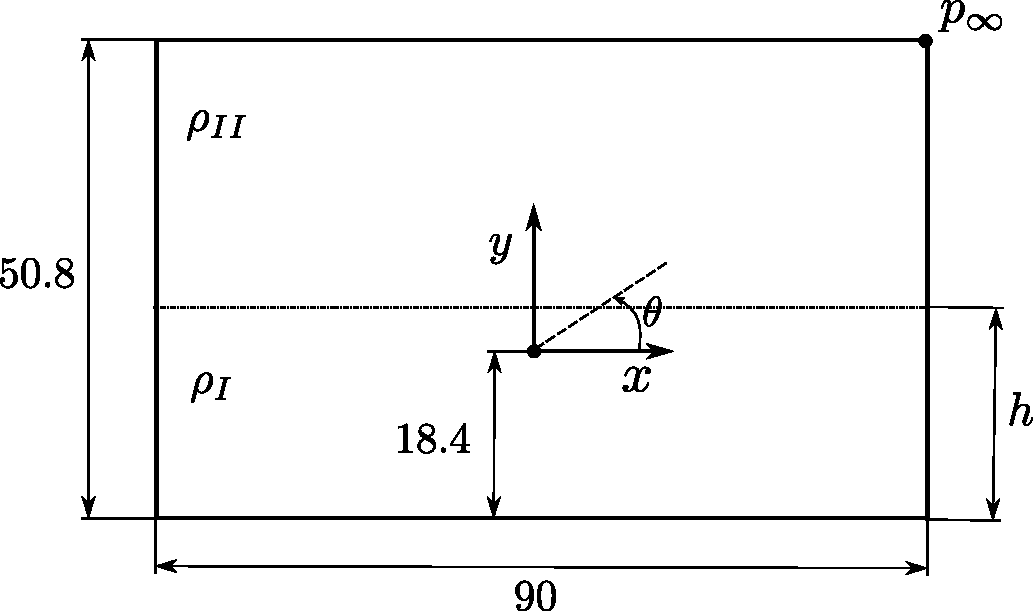
\includegraphics[width=.75\columnwidth]{images/sloshing_roll.pdf}
  \end{center}
  \caption{\label{fg:roll-config} Configuration scheme of non-linear sloshing with harmonic rolling motion. Dimensions are in centimeters.}
\end{figure}

Computational grid used is composed with $180$ by $102$ nodes conforming a mesh with around $40000$ triangles. Boundary conditions are slip on each wall, and the initial condition is water at rest with $h=22.2[cm]$. The incompressible non-viscous multifluids PFEM solver with $\rho_{I}=1000[kg/m^3]$, $\rho_{II}=1000[kg/m^3]$ and $p_{\infty}=0[Pa]$ is used, choosing a time-step $\Delta t=0.01$.

Computational grid used is composed with $270$ by $153$ nodes conforming a mesh with around $84000$ triangles. Boundary conditions are slip on each wall, and the initial condition is water at rest with $h=22.2[cm]$. The incompressible non-viscous multifluids PFEM solver with $\rho_{I}=1000[kg/m^3]$ and $\rho_{II}=1000[kg/m^3]$ is used, choosing a time-step $\Delta t=0.01$.